\documentclass[letterpaper,12pt]{article}
\usepackage[utf8]{inputenc}

\usepackage{rotating}
\usepackage[top=1in, bottom=1in, left=1in, right=1in]{geometry}
\usepackage{graphicx}
\usepackage[numbers,square,sort&compress]{natbib}
\usepackage{setspace}
\usepackage[cdot,mediumqspace,]{SIunits}
\usepackage{hyperref}
\usepackage{mathtools}
\usepackage{url}
\usepackage{authblk}
\usepackage{placeins}
\usepackage{float}

\onehalfspacing
\title{Functional Analysis: Interpolation}
\author{Anita Bahmanyar}
\affil{\small {Student Number: 998909098}}
\affil{\small {anita.bahmanyar@mail.utoronto.ca}}
\date{December 19, 2014}

\usepackage{graphicx}

\renewcommand\thesubsection{\alph{subsection}}

\begin{document}

\maketitle

\section{Introduction}
It is common to know the value of a function at a few points and wanting to know the value of the function at the points in between. Interpolation is the name given to the method for finding such a value. This is similar to passing a curve from some points provided. There is one other case where interpolation becomes handy. Some of the python built-in functions such as quad which is for integrating functions only gets single values. If we want to pass an array to the quad function it would raise an error. In that case, it is easier to pass some of the values from the quad function and interpolate the values in between the points so that we may pass arrays to the function.

\section{Interpolation Types}
\subsection{Linear Interpolation}
Linear interpolation is the simplest way of getting the values of a function in between points. Linear interpolation is a method to fit a curve to the points using linear functions. If we know the coordinates of two points as $A=(x_0,y_0)$ and $B=(x_1,y_1)$, the linear interpolation between these two points would simply be a straight line. Figure 1 shows the schematic view of the interpolation.

%figure 1
\FloatBarrier
\begin{figure}[H]
\centering
\includegraphics[scale=0.5]{linear_plot.png}
\caption{Linear interpolation gives the value of point $C=(x_2,y_2)$.}
\end{figure}
\FloatBarrier
The equation of a straight line is given by:
\begin{equation}
y = y_0 +\frac{x-x_0}{x_1-x_0}
\end{equation}
Therefore, having the values of the points A and B, we can compute the value of $y_2$ given the value of $x_2$.
This can be considered as the weighted average. The weights are inversely related to the distance from the end points to the unknown point; the closer point has more influence than the farther point. 
Since this method only returns equation of lines in between each two points, the more the number of points available, the better the linear interpolation would be.
The points are simply joined by straight line segments resulting in discontinuities at each point. 

%figure 2
\FloatBarrier
\begin{figure}[H]
\centering
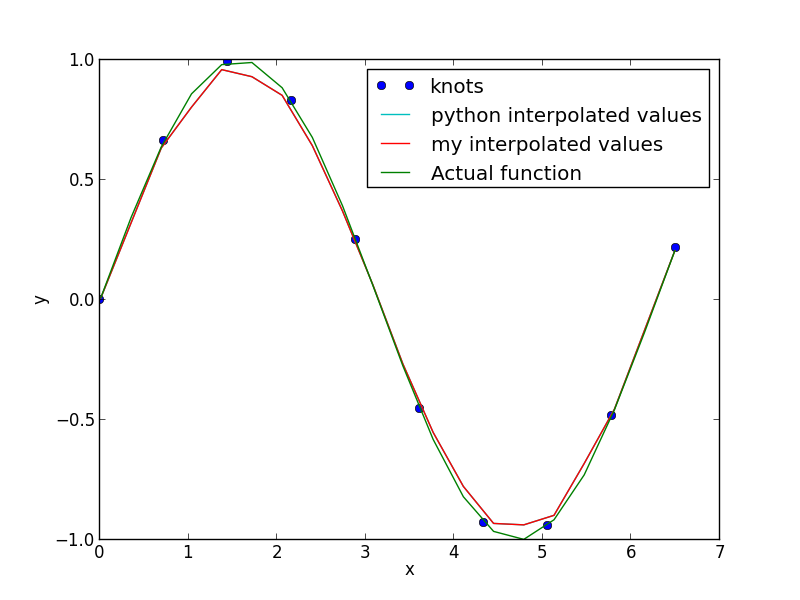
\includegraphics[scale=0.5]{lin_sin.png}
\caption{The interpolated values from my code and scipy module are very similar that they go on top of one another. This included 10 knots.}
\end{figure}
\FloatBarrier
The interpolated values using Scipy linear 1d interpolation is very similar to the values I got from my linear interpolation code.The mean value of the difference between the Python linear interpolation and my interpolation method is $\sim 1.735 \times 10^{-17}$. Linear interpolation just gives us an overall shape of the function, it is not very accurate since it only uses straight lines between each points, so it would not be a smooth function. However, as we add more knots it would seem smoother and more similar to the actual function.

%figure 2
\FloatBarrier
\begin{figure}[H]
\centering
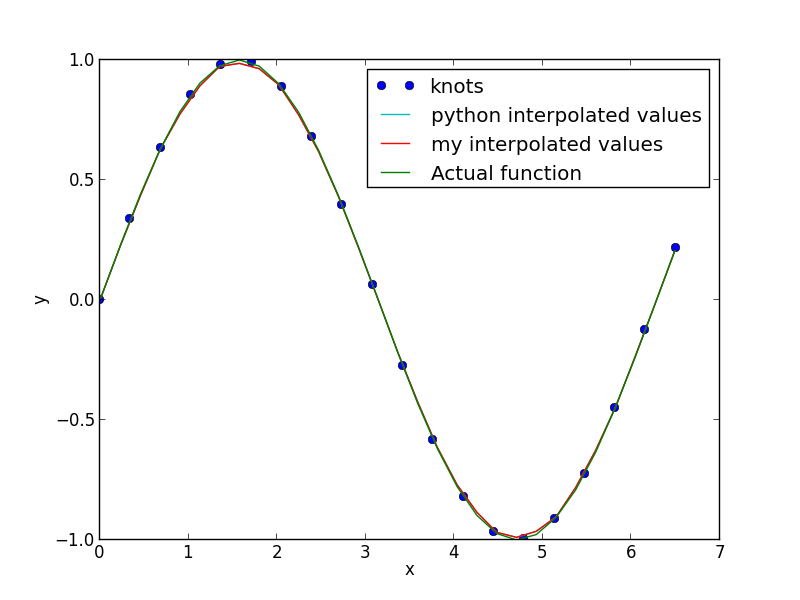
\includegraphics[scale=0.5]{lin_sin_morepoints.png}
\caption{The interpolated values from my code and scipy module are very similar that they go on top of one another. This is similar to previous figure except this is with more knots. This has 20 knots rather than 10 in the previous figure. We can see that the interpolated curves are getting closer to the function.}
\end{figure}
\FloatBarrier
Figure 3 shows that as we add more knots, the interpolated curves get more similar to the function because the line segments get smaller and more accurate between points with increasing number of knots.

\subsection{Cubic Spline Interpolation}
Cubic spline interpolation is a more accurate and advanced way of fitting a curve to data points than the linear interpolation. We need to make sure the curves passing through the points have continuous second derivative at the knots. For this purpose, we need to use polynomials that are of order 3 or higher and that is where cubic spline name comes from.

%figure 3
\FloatBarrier
\begin{figure}[H]
\centering
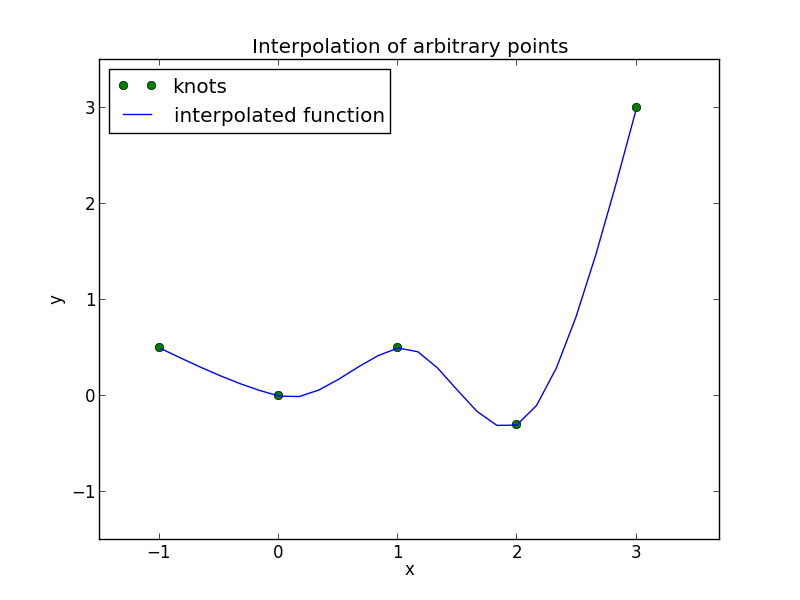
\includegraphics[scale=0.5]{interp_arbitrary.png}
\caption{Interpolation of 5 arbitrary points using cubic spline method.}
\end{figure}
\FloatBarrier

\subsubsection{Mathematical Approach}
The aim is to fit a curve passing through points $(x_i,y_i)$ where $i=0,1,...,n$, so we interpolate between points $(x_{i-1},y_{i-1})$ and $(x_i,y_i)$ with polynomials $y_i = q_i(x)$.



In order to have continuous function at all the knots the following condition holds:
%equation
\begin{equation}
\frac{k_{i-1}}{x_i - x_{i-1}} +    \left (    \frac{1}{x_i - x_{i-1}} + \frac{1}{x_{i+1}-x_i} \right ) 2k_i + \frac{k_{i+1}}{x_{i+1}-x_i} = 3  \left(  \frac{y_i - y_{i-1}}{(x_i - x_{i-1})^2} + \frac{y_{i+1}-y_i}{( x_{i+1}-x_i )^2} \right)
\end{equation}
for $i=1,2,...,n-1$. This gives us $n-1$ equations including $k_0$, $k_1$, ..., $k_n$.

For the two knots at both ends, the condition is different and we have:
%equation
\begin{equation}
\frac{2}{x_1-x_0}k_0 + \frac{1}{x_1-x_0}k_1 = 3\frac{y_1-y_0}{(x_1-x_0)^2}
\end{equation}


%equation
\begin{equation}
\frac{1}{x_n-x_{n-1}}k_{n-1} + \frac{2}{x_n-x_{n-1}}k_n = 3\frac{y_n-y_{n-1}}{(x_n-x_{n-1})^2}
\end{equation}

These two equations give us 2 more equations and along with the previous $n-1$ equations we would have $n+1$ equations to solve for $k_0$,$k_1$,..,$k_n$ values. The cubic spline�s coefficients can be found by solving a tridiagonal linear system. 
%equation, matrix form
\begin{equation}
\begin{bmatrix}
a_{11} & a_{12} & &  &  & &\\ 
a_{21} & a_{22} & a_{23} & &  & &\\ 
 & a_{31} & a_{32} & a_{33} & & &\\
 &  & \ddots & \ddots & \ddots& &\\ 
 &  & & a_{n-1n-2}& a_{n-1n-1}&a_{n-1n}\\ 
 &  & & & a_{nn-1} & a_{nn}  
\end{bmatrix}
\begin{bmatrix}
k_0\\ 
k_1\\ 
k_2\\ 
\vdots\\ 
k_{n-1}\\
k_n\\
\end{bmatrix} = 
\begin{bmatrix}
b_0\\ 
b_1\\ 
b_2\\ 
\vdots\\ 
b_{n-1}\\
b_n \\
\end{bmatrix}
\end{equation}

Then having the values of $k_i$, we can calculate $a_i$ and $b_i$ values:
%equation
\begin{equation}
a_i = k_{i-1} (x_i-x_{i-1}) - (y_i - y_{i-1})
\end{equation}

%equation
\begin{equation}
b_i = -k_i (x_i - x_{i-1}) + (y_i - y_{i-1})
\end{equation}
and use these values to calculate $q_i$ values:

%equation
\begin{equation}
q_i = (1-t)y_{i_1} + ty_i + t(1-t) (a_i (1-t) +b_it)
\end{equation}
where t is:

%equation
\begin{equation}
t = \frac{x-x_{i-1}}{x_i - x_{i-1}}
\end{equation}

This will give us a function q for the points between each two knots, so we will have n different functions for the n+1 knots.


\subsubsection{Error Analysis}
The error in cubic spline interpolation is of order $O(h^4)$. The error would be the maximum difference between the value of the function we are approximating and our interpolated value. The error in cubic spline is given by:
\begin{equation}
\left | s-f \right | \sim \frac{5}{384}. \left | f^{(4)} \right |. h^4
\end{equation}
where $s-f$ is the difference between interpolated and the function value, $f^{(4)}$ is the value of fourth derivative of the function and h is the spacing between knots.
For example, if we do the interpolation on the function $y(x) = \sin(x)$ over the interval [0,3] with $h$= 0.1, what would the error be?
\\We know $f^{(4)}(x)$ = $\sin(x)$; therefore, $f^{(4)}(x) \leq$ 1. So the value of the error would be:
\\ $\frac{5}{384}.1.(0.1)^4$ $\approx$ $\frac{1}{768000} \approx 1.3 \times 10^{-6}$. This error is very small so the cubic spline interpolation is a good approximation of the function. 

Now to see how good it works, I have applied the code to do the interpolation for the function $\sin(x)$ in the interval [0,6.5] with 20 points, so $h$ = 0.325 here. So the error would be $\sim 1.46 \times 10^{-4}$. This is still quite a small error.

\subsection{Bilinear Interpolation}
Bilinear interpolation is the same as linear interpolation which is extended into two dimensions. Unlike 1D interpolation where you entered $x$ values and got $y=f(x)$ values out, this would require you to enter $x$ and $y$ values to get the value of the function $z = f(x,y)$ out. Figure 5 shows a schematic view of bilinear interpolation.

%figure 5
\FloatBarrier
\begin{figure}[H]
\centering
\includegraphics[scale=0.5]{bilinear_plot.png}
\caption{The red points show the knots and the green point P is the point we want its value.}
\end{figure}
\FloatBarrier


\subsubsection{Mathematical Approach}
The four points indicated by red dots in figure 5 have the values of:
\\$Q_{11} = (x_1,y_1)$, $Q_{12} = (x_1,y_2)$, $Q_{21} = (x_2,y_1)$ and $Q_{22} = (x_2,y_2)$. Also, the blue dots in figure 5 are $R_1=(x,y_1)$ and $R_2=(x,y_2)$. The green dot is the point where we want to find the value $P=(x,y)$.
\\Doing linear interpolation in x-direction first would give us:
\begin{equation}
f(R_1) \approx \frac{x_2-x}{x_2-x_1}f(Q_{11}) + \frac{x-x_1}{x_2-x_1}f(Q_{21})
\end{equation}
and
\begin{equation}
f(R_2) \approx  \frac{x_2-x}{x_2-x_1}f(Q_{12}) + \frac{x-x_1}{x_2-x_1}f(Q_{22})
\end{equation}
Then we continue the interpolation in y direction which gives u:
\begin{equation}
f(P) \approx \frac{y_2-y}{y_2-y_1}f(R_1) + \frac{y-y_!}{y_2-y_1}f(R_2)
\end{equation}
Finally, the estimate of the interpolated function would be:
\begin{eqnarray}
f(x,y) \approx \frac{1}{(x_2-x_1)(y_2-y_1)} \left ( f(Q_{11})(x_2-x)(y_2-y) + 
\\f(Q_{21})(x-x_1)(y_2-y) + 
\\f(Q_{12})(x_2-x)(y-y_1) + 
\\f(Q_{22})(x-x_1)(y-y_1) )\right)
\end{eqnarray}
This could have been done by doing the linear interpolation first in y direction and then in x direction without any change in the result. This kind of interpolation is linear in x and in y direction separately but not as a whole despite its name.

%figure of colours
\FloatBarrier
\begin{figure}[H]
\centering
\includegraphics[scale=0.5]{bilinear_plot2.png}
\caption{The value of the function at point $P=(x,y)$ is the value of each coloured point multiplied by the area of the same colour divided by the area of ABCD rectangle to normalize it.}
\end{figure}
\FloatBarrier
\section{Analysis}

\subsection{Code Analysis}
As you can see in figure 1, the Python built-in interpolation function does a better job in cubic spline interpolation than my code. The zoomed in figure shows that my interpolation is still very close to the actual function even though it differs a bit from the function and the python interpolated function.
\\Figure 6 shows another schematic view of bilinear interpolation to demonstrate the mathematical part of it better.
%figure 2	
\FloatBarrier
\begin{figure}[H]
\centering
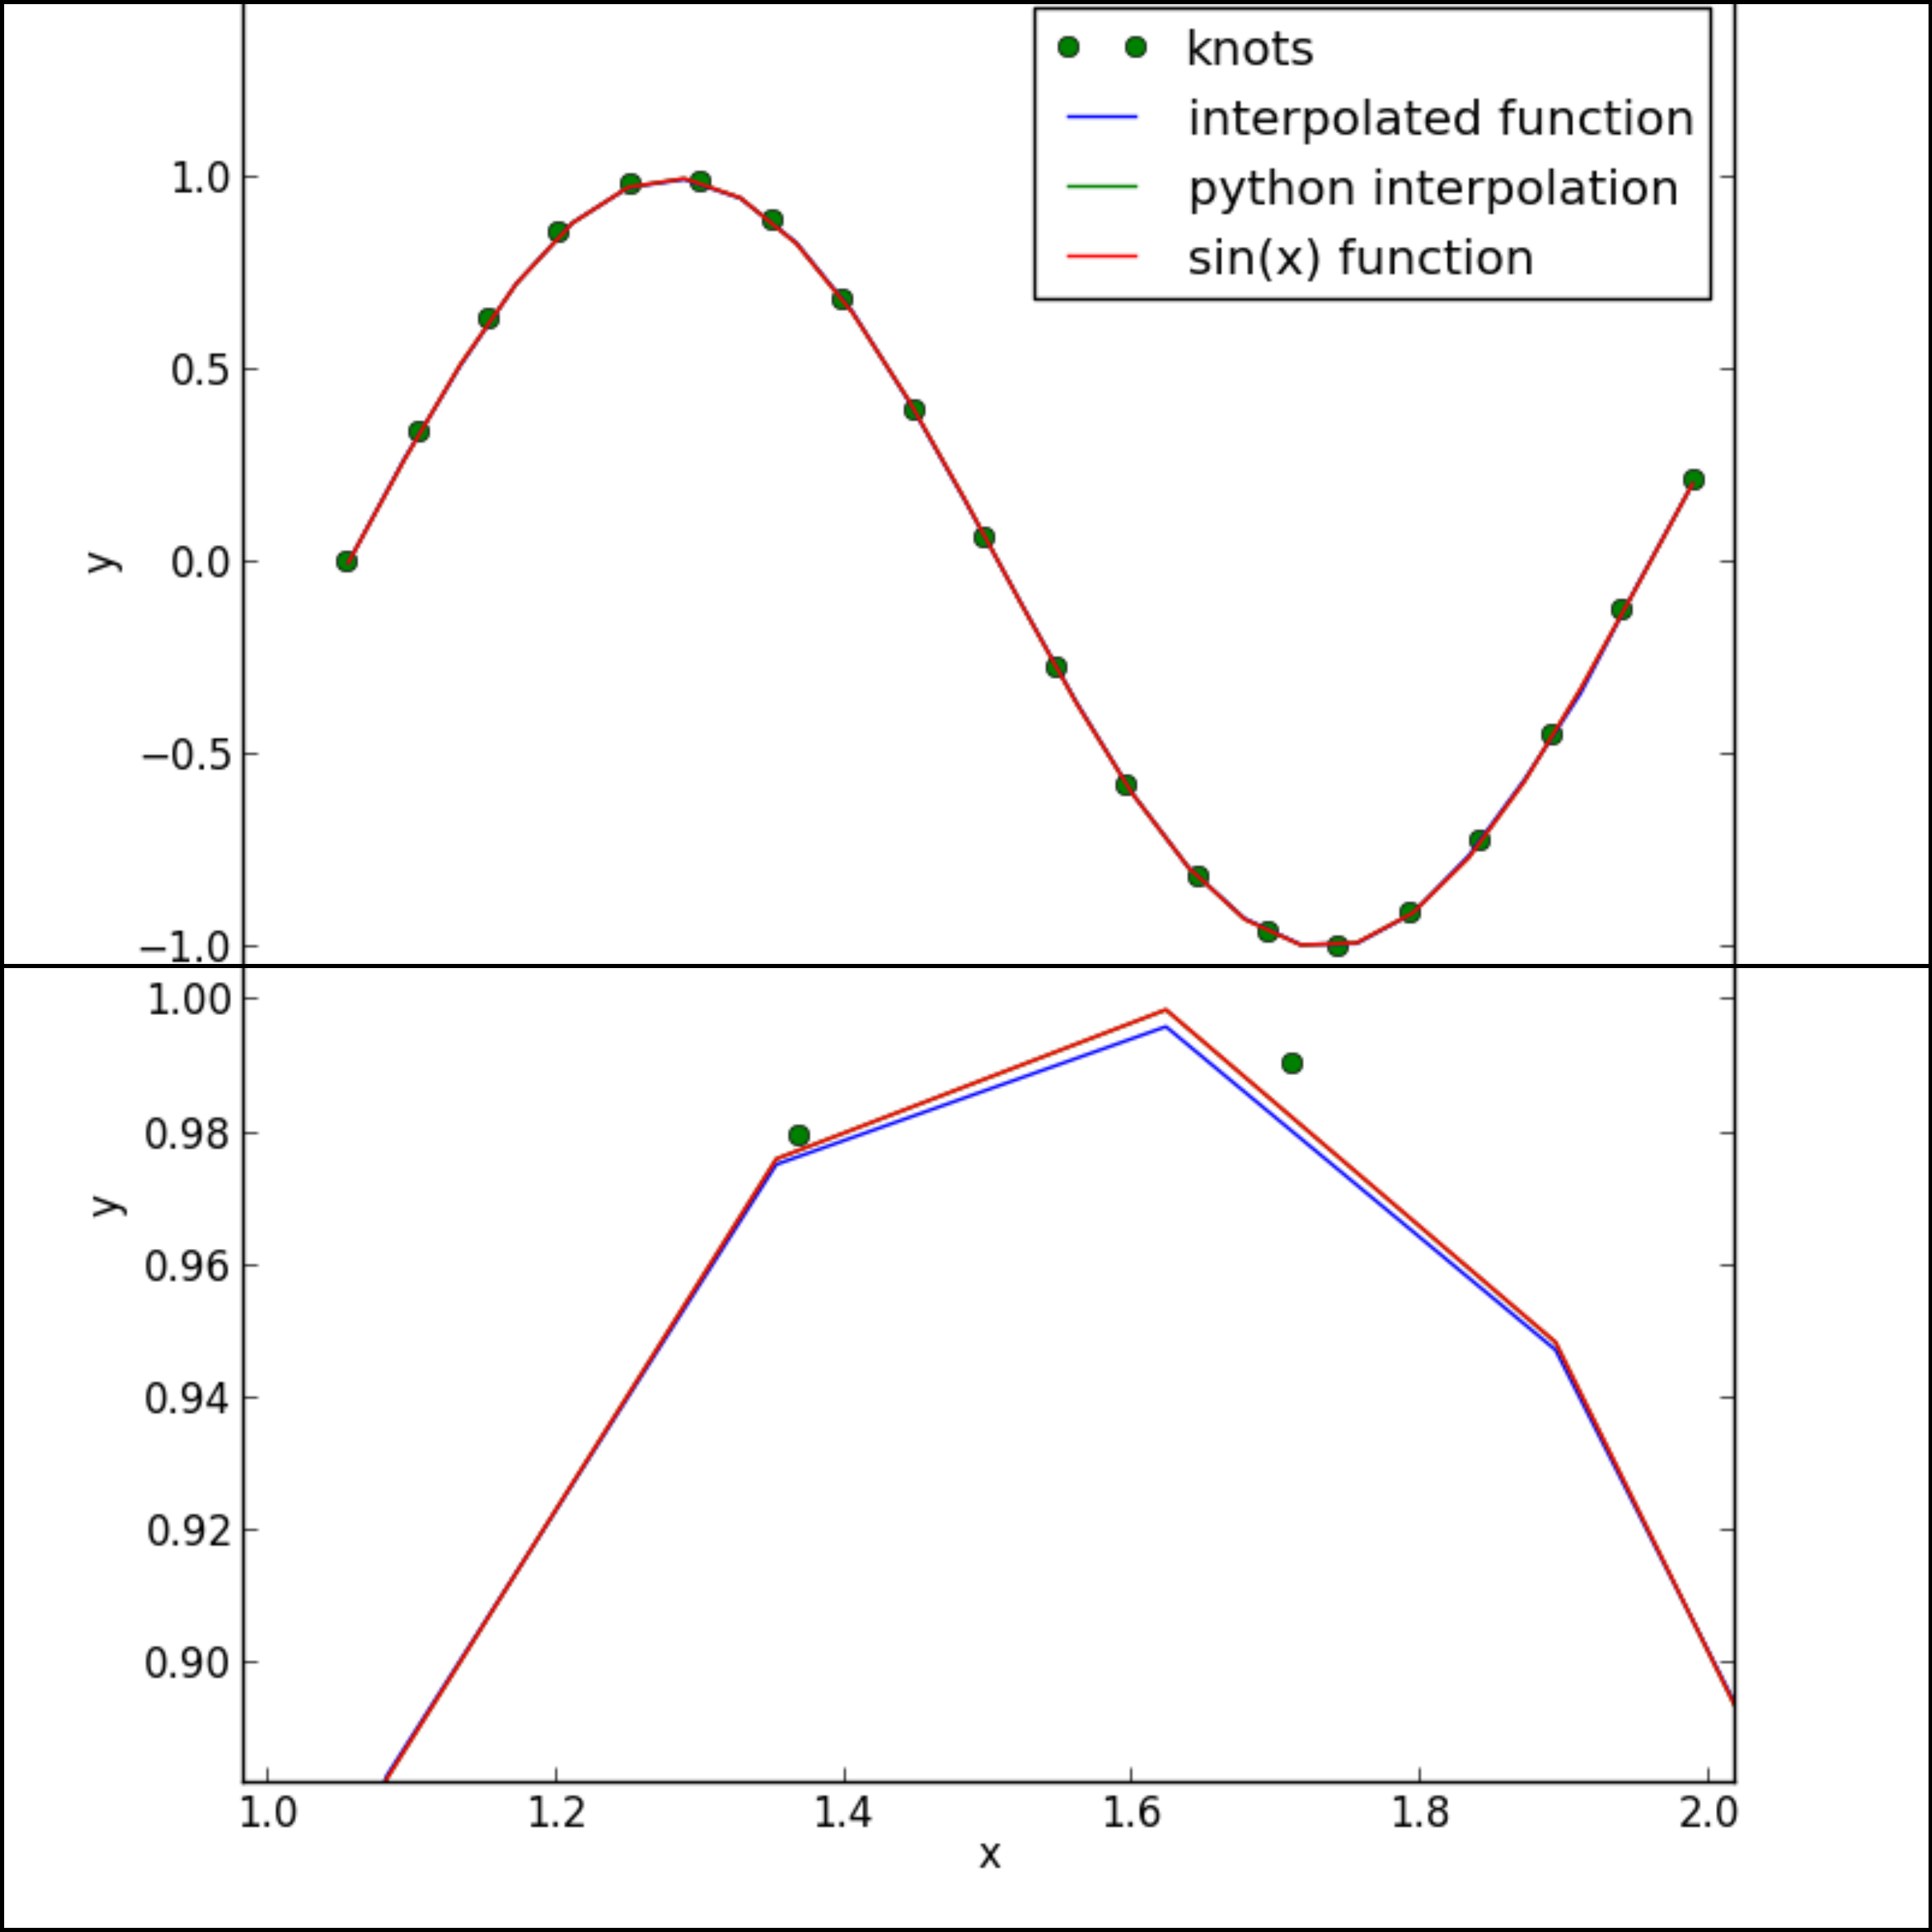
\includegraphics[scale=0.1]{cubic_compared_final.png}
\caption{Upper: Knots are shown in green dots, red is the actual sin(x) function and blue and green are my interpolated function and Python built-in interpolation function, respectively. Lower: Zoomed in version of the figure above. Python built-in function does a better job in cubic spline interpolation.}
\end{figure}
\FloatBarrier

\section{References}
1-http://bmia.bmt.tue.nl/people/BRomeny/Courses/8C080/Interpolation.pdf
\\2-http://en.wikipedia.org/wiki/Linear\_interpolation
\\3-http://en.wikipedia.org/wiki/Bilinear\_interpolation
\\4-http://en.wikipedia.org/wiki/Spline\_interpolation

\end{document}


